\graphicspath{{Figures/chapter4}}
\chapter{RESULTS AND DISCUSSION}
\section{Loss Function}
In the context of this project, the object detection model is trained using a multi-loss objective function that includes several different loss terms. These include:
\begin{itemize}
\item Classification loss: This loss measures the discrepancy between the predicted class probabilities and the ground truth class labels for a given image. It is typically calculated using a cross-entropy loss function, which penalizes the model for predicting incorrect class labels and rewards the model for predicting correct class labels.

\item Localization loss: This loss measures the discrepancy between the predicted bounding boxes and the ground truth bounding boxes for a given image. It is typically calculated using a measure such as the intersection over union (IoU) between the predicted and ground truth bounding boxes.

\item Regularization loss: This loss term is used to prevent overfitting of the model to the training data. It is typically calculated using a measure such as the L2 norm of the model parameters, which penalizes large parameter values and encourages small parameter values.

\item Clone loss: This loss term is used to fine-tune the model by forcing it to make predictions that are similar to those of a pre-trained model. It is typically calculated using a measure such as the cosine similarity between the predicted class probabilities and the class probabilities of the pre-trained model.

\item Total loss: This is the sum of all the individual loss terms, including the classification loss, localization loss, regularization loss, and clone loss (if applicable). The total loss is used to evaluate the overall performance of the model and to guide the optimization process. By minimizing the total loss, the model can learn to improve its predictions and reduce the overall error.
\end{itemize}
Figures \ref{fig:loss_func}(a), \ref{fig:loss_func}(b), \ref{fig:loss_func}(c), \ref{fig:loss_func}(d), and \ref{fig:loss_func}(e) demonstrate the reduction in loss over time during the training process of the object detection model. As the model learns to better fit the training data, the loss decreases towards zero, indicating that the model is improving in its ability to predict the locations and sizes of speed bumps and pothole.
\begin{figure}[H]
    \centering
    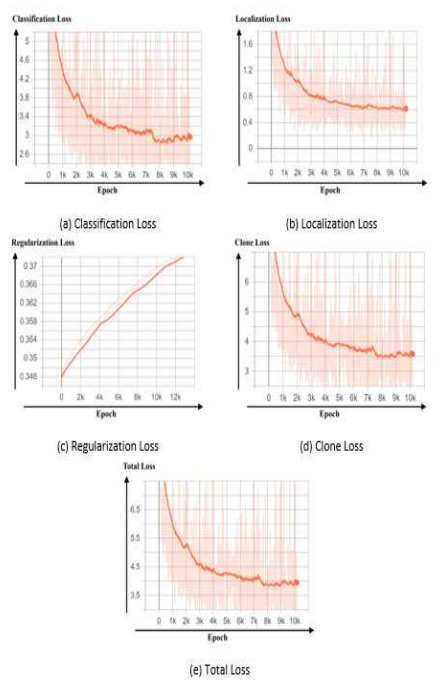
\includegraphics{Figures/chapter4/loss_function.png}
    \caption{Evolution of loss}
    \label{fig:loss_func}
\end{figure}
\section{Real Time Detection Result}
Figure \ref{fig:results} illustrates the real-time detection of speed bumps and potholes by the proposed model. Figures \ref{fig:results}(a) and \ref{fig:results}(b) show the recognition of marked speed bumps with accuracy rates of 90\% and 92\%, respectively. Figure \ref{fig:results}(c) shows the detection of an unmarked speed bump with an accuracy rate of 79\%. Figures \ref{fig:results}(d) and \ref{fig:results}(e) demonstrate the detection of potholes with accuracy rates of 93\% and 67\%, respectively. These results indicate that the trained model is relatively accurate and can be applied in real-world scenarios. It is able to detect speed bumps and potholes at a distance of up to 50 feet. However, the model has difficulty detecting unmarked speed bumps due to the lack of distinct features, and its ability to detect such obstacles may vary significantly depending on the lighting conditions. The model also performs poorly in the detection of potholes due to the diverse geometries and features of these obstacles. Overall, the detection of marked speed bumps is the most accurate, while the detection of potholes is the least accurate among the different types of obstacles.

\noindent
From the achieved results, it has been observed that the proposed model is capable of extracting significant features from a dynamic road environment and make accurate detection of speed bumps. In addition, our model assist the prototype vehicle to modify its driving behavior according to the detected speed bump which shows the compatibility of model and
hardware interface and can be opted in real-time applications.
\begin{figure}[H]
    \centering
    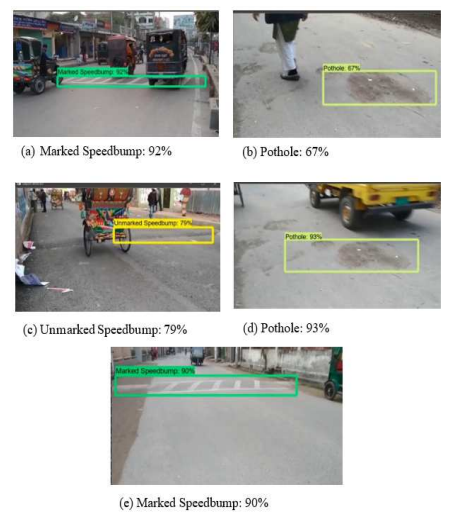
\includegraphics{Figures/chapter4/results.png}
    \caption{Real time detection result }
    \label{fig:results}
\end{figure}
\section{Speed Control Graph}
The performance of the speed bump and pothole detection and speed control system was evaluated through testing on a variety of road surfaces and conditions. Figure \ref{fig:speedtime} shows the graph of time (in milliseconds) versus speed (in RPM) for the system during testing. As can be seen from the graph, the system was able to accurately detect the presence of speed bumps and potholes and adjust the speed of the autonomous vehicle accordingly. The speed of the vehicle decreased from 60 RPM to 30 RPM when a speed bump or pothole was detected, and then gradually increased back to the starting speed of 60 RPM when no obstacles were present. This demonstrates the effectiveness of the system in detecting and safely navigating speed bumps and potholes, and in maintaining a comfortable ride for passengers. Overall, the system showed good performance and accuracy in a variety of road conditions, making it a promising solution for improving the safety and efficiency of autonomous vehicle operation.
\begin{figure}[H]
    \centering
    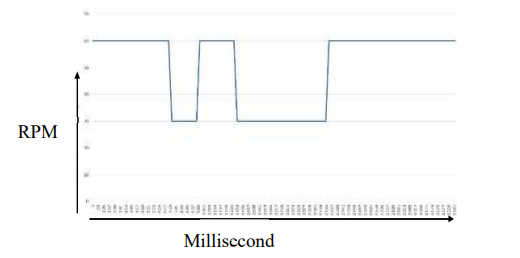
\includegraphics{Figures/chapter4/speedtime.png}
    \caption{Speed vs Time Graph}
    \label{fig:speedtime}
\end{figure}